\section{Experimental setup and measurements}
\label{sec:Experimentale}
The experiment is conducted by using the Sagnac-Interferometer introduced in \ref{subsec:Sagnac_Interferometer}. 
The topology of the interferometer can be seen in \autoref{pic:Sagnac-Interferometer}.As a 
source of light a Helium-Neon laser is used. The plane of the linear polarized laser beam is tilted about $45°$ in comparison to 
the vertical. This leads to the beam being split into two beams of the same intensity and perpendicular polarization by the PBSC.
In front of the PBSC a polarisation filter is placed so the incomming beam is traveling through the filter and afterwards through the 
PBSC. 

\begin{figure}
    \centering
    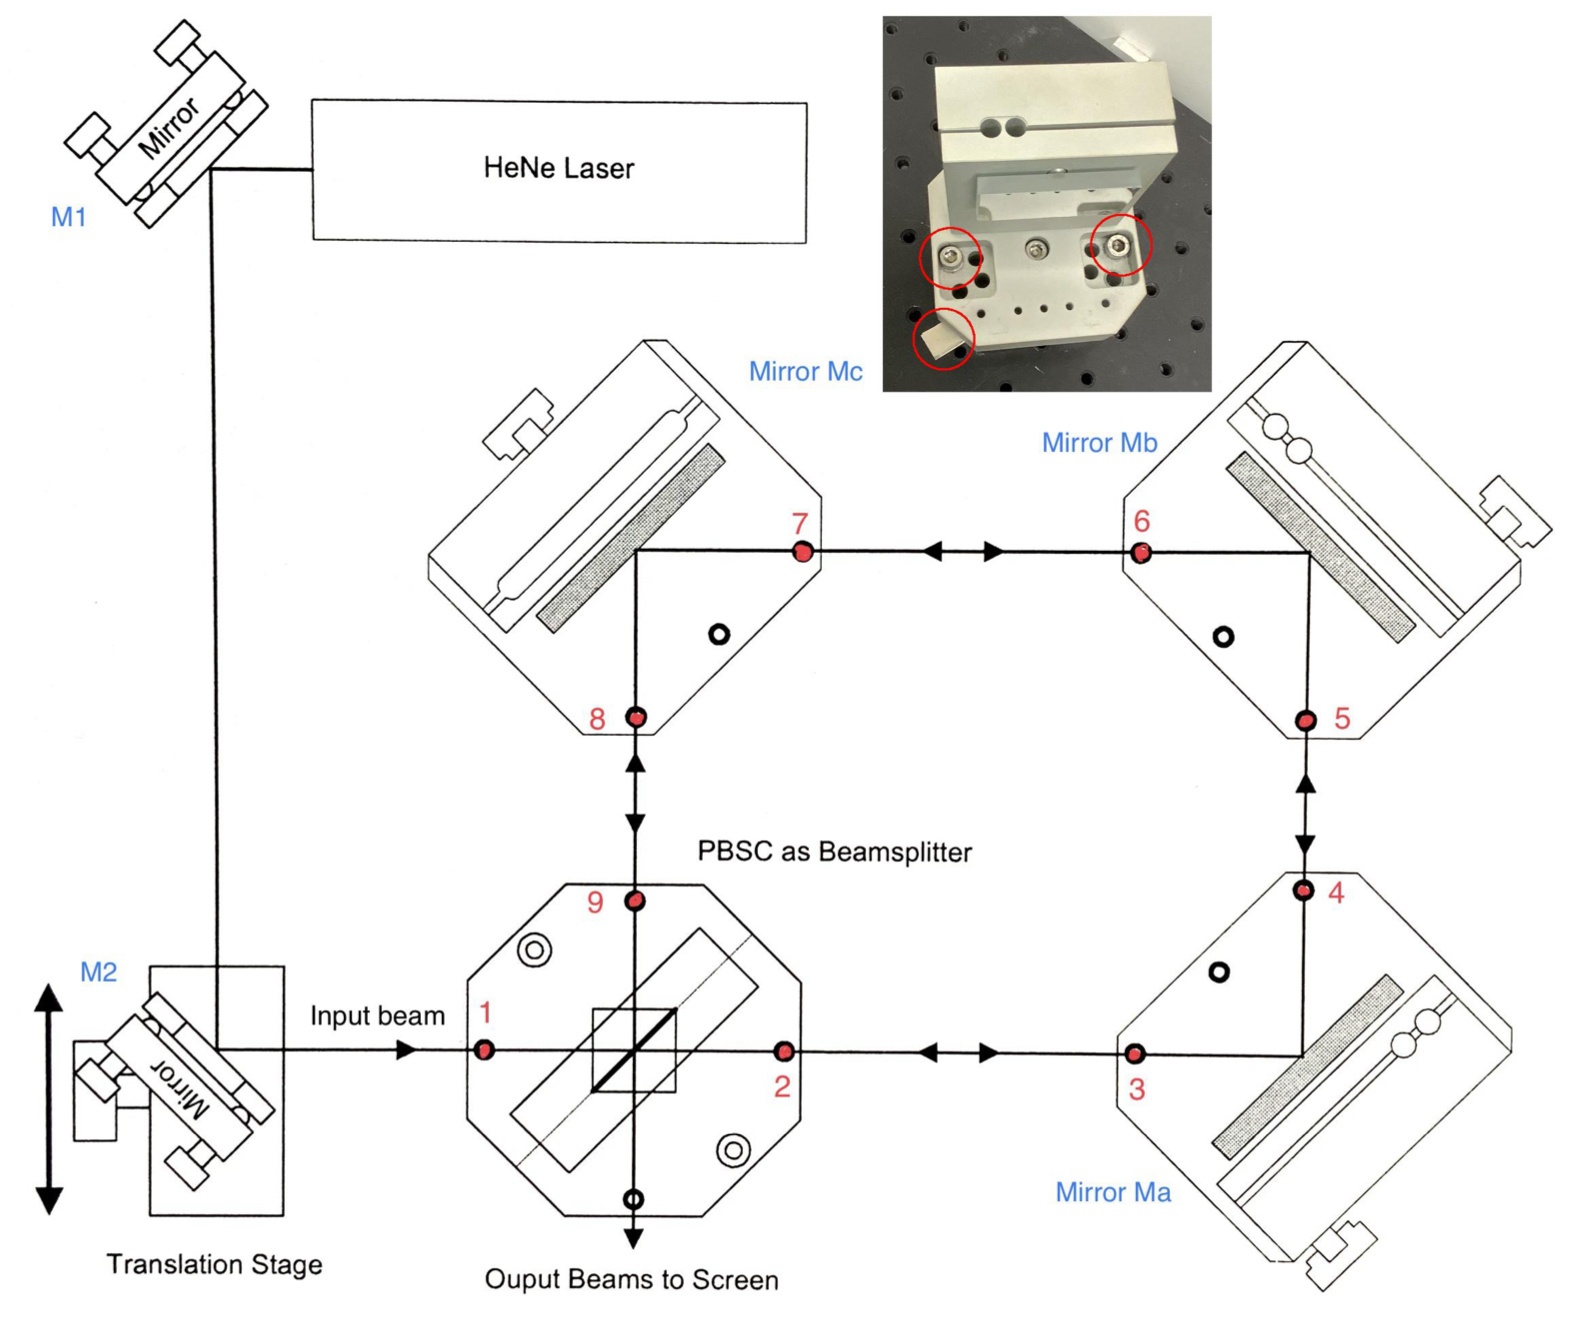
\includegraphics[width=0.70\textwidth]{content/Bilder/Sagnac_Interferometer.jpeg}
    \caption{Topology of the Sagnac-Interferometer}
    \label{pic:Sagnac-Interferometer}
  \end{figure}

To make the interference of the two beams possible the beams must travel through a polarization filter to create an overlapping polarization. 

\subsection{Alignment}
The correct alignment is a critical part of the experiment. For the interference to work the beams have to be parallel to each over and 
overlap at all times. This is achieved by using adjustment plated which have holes at the top where the beam should travel through. 
